\chapter[Wheelchair locomotion]{Analysis of manual wheelchair locomotion}
\label{locomotion_analysis}
%\minitoc
\section{Introduction}
Wheelchair locomotion concerns many people, for different reasons: genetic  (myopathy), accidental (spinal cord injury, lower extremity amputee), degenerative (multiple sclerosis, poliomyelitis) or just related to the natural aging of locomotor functions (muscle degeneration, arthritis of the lower limbs, etc.). Then, in the 34 developed countries, it is estimated that 1\% or 10,000,000 people require a wheelchair. In the 156 developing countries, it is estimated that at least 2\% or 121,800,000 people require a wheelchair. Overall, of the 7,091,500,000 people in the world, approximately 131,800,000 or 1.85\% need a wheelchair \cite{Needs2016}. However, the use of manual wheelchair is not without risk.

\section[Problem]{The problem of locomotion manual wheelchair locomotion}
\label{problem}
Although the wheelchair use improves the mobility of its users, doctors quickly realized that it often leads to sedentarization, and to related problems of obesity, diabetes, etc. Also, to promote daily physical activity, sport has been strongly encouraged \cite{machida2013resilience}. However, intensive and prolonged sports practice in Manual WheelChair (MWC) can lead to specific injuries and pains \cite{johnson2004sport}, especially in the shoulder, and at the elbow, wrist and hand. For instance in \cite{pentland1991weight}, the  authors claimed that 73\%  of paraplegic individuals suffered from shoulder pain. In addition, prolonged sitting of   users causes dermatological problems such as bedsores or pressure ulcers, due to immobility, loss of sensitivity and incontinence. These symptoms are recognized as a major cause of discontinuation of wheelchair use \cite{van2006manual}  \cite{ville2006work}, thus the sedentarization of users.  \cite{lundqvist1991spinal} showed that upper limb pain was the main factor correlated with poor quality of life in MWC users. The challenge for the therapist is then to encourage a daily practice of physical activity adapted to  wheelchair users, for limiting orthopedic problems,  and thus to promote the use of the MWC over time.


Given the problems faced by manual wheelchair users at the level of
their autonomy and health, van der Woude et al. \cite{van2005wheelchair} \cite{woude1986wheelchair} summarized the issues of manual wheelchair locomotion research into three main areas:

\begin{itemize}
\item Improving the interface between the subject and his manual wheelchair, that is, the ergonomy and the adequacy of the system \{subject + MWC\} with the external physical environment (ramps, lifts, corridor widths, etc.).
\item The improvement of the MWC regarding the design and the mechanical principles of propulsion;
\item \textbf{Improving the subject's physical abilities}, that is, improving propulsion techniques, as well as rehabilitation techniques and training programs.
\end{itemize}

After the construction of a measuring tool,  a wheelchair field ergometer \ref{dabonneville2005self},  bio-mechanical works has been conducted in LIMOS to identify and quantify traumatic factors such as \cite{Remy2005}  \cite{Sauret2010}. 

\section[Evaluation tools]{Tools to evaluate manual wheelchair locomotion}
\label{measurment_tools}
This section summarises different tools designed over the last 60 years to measure the efforts made by subjects moving in a MWC. We put a  particular emphasis on the wheelchair  ergometer designed and manufactured at LIMOS, which is at the origin of the time series that are the subject of our analysis throughout this thesis.

\subsection{Crank Ergometers}
Crank ergometers allow a subject to manually operate a crankset connected to the flywheel of an ergo-cycle. The speed is determined by measuring the rotation speed of the flywheel, whose diameter is known, or by imposing a cadence, in which case the rotation speed is considered constant. Crank ergometers established that the mechanical work of the upper limbs is less efficient than that of the lower limbs and also that the physical capacities evaluated by the maximum oxygen consumption of MWC users depended on their level of spinal injury (cervical, thoracic or lumbar injury)\footnote{This assertion will be commented later in chapter \ref{chapter_saxp}}. One of the main limitations of crank ergometers is that the motion measured from a crank ergometer is not representative of the MWC propulsion motion, most of which is propelled by handrims \cite{0aastrand1961maximal}  \cite{bergh1976maximal}    \cite{stenberg1967hemodynamic}.

\subsection{Roller Ergometers}
To reproduce more precisely the specificities of  MWC locomotion, Brouha and Krobathc\cite{brouha1967continuous}, as early as 1967, used a roller ergometer to measure cardiac and respiratory responses during continuous MWC exercice. This tool consisted of a platform on which were fixed two rollers, each rotating around an axis and on which rested the rear wheels of a real MWC. The MWC frame was attached to the ergometer, and the subjects simulated locomotion by applying forces to the handrims, causing the rear wheels of the MWC and the rollers to rotate. 


In 1971, Stoboy et al. \cite{stoboy1971workload}, using an ergometer inspired by that of Brouha and Krobath, quantified the mechanical power (in watts) produced by the user from the relationship between oxygen consumption and mechanical power calculated during an incremental exercise on a crank ergometer.


The problem with roller ergometers of \cite{brouha1967continuous}\\\cite{stoboy1971workload} was that they did not take into account the influence of the inertia of translation encountered by the Subject when he moves. To take this phenomenon into account, the rollers have been connected  to a small flywheel. However,  both rear wheels were on the same rollers, which did not allow to measure the differences in propulsion between the right and left wheels to be explored \cite{brouha1967continuous} \cite{stoboy1971workload}.



Then \cite{langbein1993research} \cite{langbein1993calibration} \cite{langbein1994initial}  designed a new roller ergometer called the Wheelchair Aerobic Fitness Trainer (WAFT), which had an access ramp to facilitate subject and MWC installation (Figure \ref{WAFT}). When the latter was attached to the ergometer, its rear wheels rested on three rollers each, which made it possible to differentiate the forces applied to the right and left wheels\footnote{This separation is essential to establish the dissymmetry of wheelchair locomotion and is discussed in more details in chapter \ref{chapter_saxp}}.

\begin{figure}[h]
\center
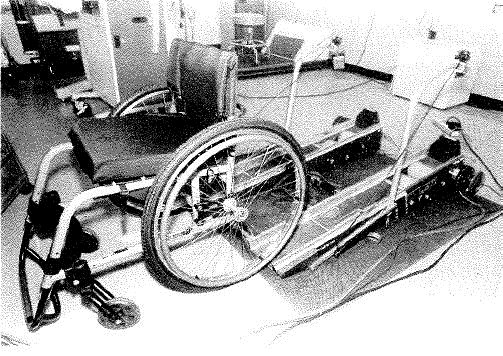
\includegraphics[scale = 25]{images/WAFT}
\caption{ Wheelchair Aerobic Fitness Trainer (WAFT) photograph \cite{langbein1993research}.}
\label{WAFT}
\end{figure}


Other roller ergometers have also been developed over the last four decades and particularly in the last fifteen years: Eagle Wheelchair Roller \cite{kerk1995effect}, Bromking Turbo Trainer \cite{goosey2001kinetic} \cite{goosey2001kinetic} \cite{ price1999thermoregulatory} or very recently the "Computer Monitored Wheelchair Dynamometer" \cite{cooper2003wheelchair}  \cite{digiovine2001dynamic}.  Other braking systems have been used, such as mechanical braking using a friction belt on a flywheel\\\cite{goosey1998relationship}  \cite{kulig2001effect} \cite{rodgers1994biomechanics}(Figure \ref{FRER}), an electric motor creating a frictional moment around the roller rotation axes \\\cite{coutts1987aerobic} \cite{kerk1995effect} \cite{patterson1997selected}     \\ \cite{vanlandewijck1999field} or an isokinetic apparatus  \cite{ruggles1994biomechanics}. To determine the speed, angular position sensors  \cite{brouha1967continuous}  \\ \cite{coutts1987aerobic}  \cite{coutts1990kinematics}  \cite{patterson1997selected} \\ \cite{rodgers1994biomechanics}, optical encoders   \cite{devillard1999wheelchair} \cite{devillard2001validation}   \\ \cite{langbein1993calibration}  \cite{langbein1994initial}  \cite{newsam1996temporal}  \\ \cite{theisen1996new}, tachometers  \cite{cooper1990exploratory}  \cite{kerk1995effect}   \cite{masse1992biomechanical} \\  \cite{vanlandewijck1999field} or speedometers   \cite{goosey1998relationship}  \cite{rodgers1994biomechanics} were used.

\begin{figure}[h]
\center
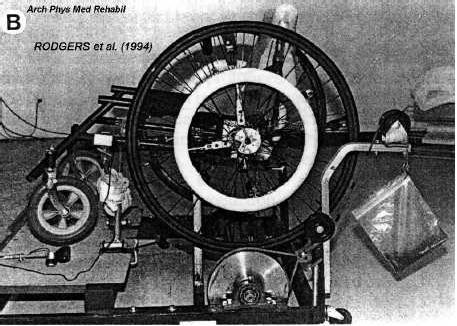
\includegraphics[scale = 25]{images/FRER}
\caption{Picture of a wheelchair on a roller ergometer with mechanical braking by friction belt on a flywheel. \cite{rodgers1994biomechanics}.}
\label{FRER}
\end{figure}

The main advantage of roller ergometers is that they allow subjects to be studied with their own MWC. Moreover, they occupy a little space in the laboratory and allow the MWC to be completely immobilized, thus ensuring the stability of the subject on the MWC and facilitating the measurement of  various physiological parameters. However, the various methods for estimating external  mechanical power used up to now still need to be refined to better evaluate this parameter. Furthermore, the comparison between the results of studies carried out with different roller ergometers and different mechanical models must be done with caution since the parameters neglected or taken into account are not all the same.

\subsection{Treadmill}
Like roller ergometers, the main advantage of treadmills is that they allow subjects to be studied with their own MWC. Since the four wheels of the MWC roll on the belt, the rolling friction forces are most certainly equivalent to those existing on the ground. Unlike roller ergometers, treadmills  allow to define a rolling speed of the belt and also a slope, that is, an inclination of the treadmill with respect to the horizontal. The main disadvantage of a treadmill comes from the steering problem related to the control of the trajectory: indeed, a subject could drift and be ejected from the treadmill; to remedy this, railings have been installed on both sides using a surface strip that limits lateral movements \cite{claremont1985model}. However, it has still not been demonstrated that the propulsion technique used was identical on a treadmill and on the ground.

\begin{figure}[h]
\center
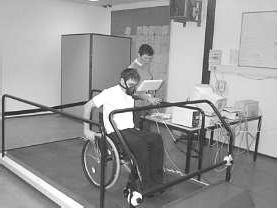
\includegraphics[scale = 40]{images/tapi_roulant}
\caption{ Exercise testing on a motor driven treadmill \cite{van2006manual}}
\label{tapi_roulant}
\end{figure}

\subsection{Wheelchair simulators}
To overcome the problems related to rolling resistance, some researchers chose to fix the rear wheels of the MWC without contact with the ground, on a rigid and fixed chassis on which the Subject could sit. The advantage of MWC simulators is that they can test different settings such as seat position or rear wheel camber angle, for example. The mechanical propulsion model is also simplified compared to roller ergometers and conveyor belts, which allows a better quantification of work and external mechanical power.   However, the influence of the Subject's movements on the seat is not taken into account. This aspect is the major disadvantage of the simulators because neither the forces of resistance to the advance nor the kinematics of the MWC is modified according to the movements of the Subject on the seat.

\begin{figure}[h]
\center
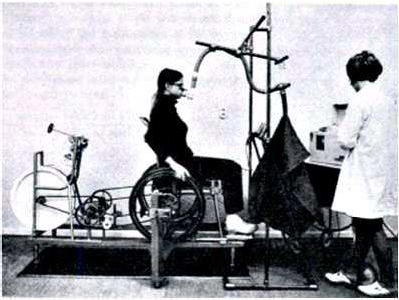
\includegraphics[scale = 30]{images/SFR}
\caption{Photograph of an experiment on a simulator connected to a flywheel (\cite{brattgaard1970energy})}
\label{SFR}
\end{figure}

\subsection{Wheelchair Field-Ergometer}
To analyse the efficiency of wheelchair propulsion, a Wireless Wheelchair Ergometer (WWE or FRET-1)  equipped with several sensors has been manufactured \cite{dabonneville2005self}. The sensors installed on the wheelchair measure the physical stresses applied to the MWC during actual use and record them.


The sensors are located on the right and left wheels of the MWC, on the footrest, on the seat and the backrest. These sensors measure the torques applied to each of the systems mentioned above.  Other sensors installed on the FRET-2 are used to measure the kinematic parameters (speed, acceleration) of the movement of the MWC (Figure \ref{fret_legend}).


\begin{figure}[h]
\center
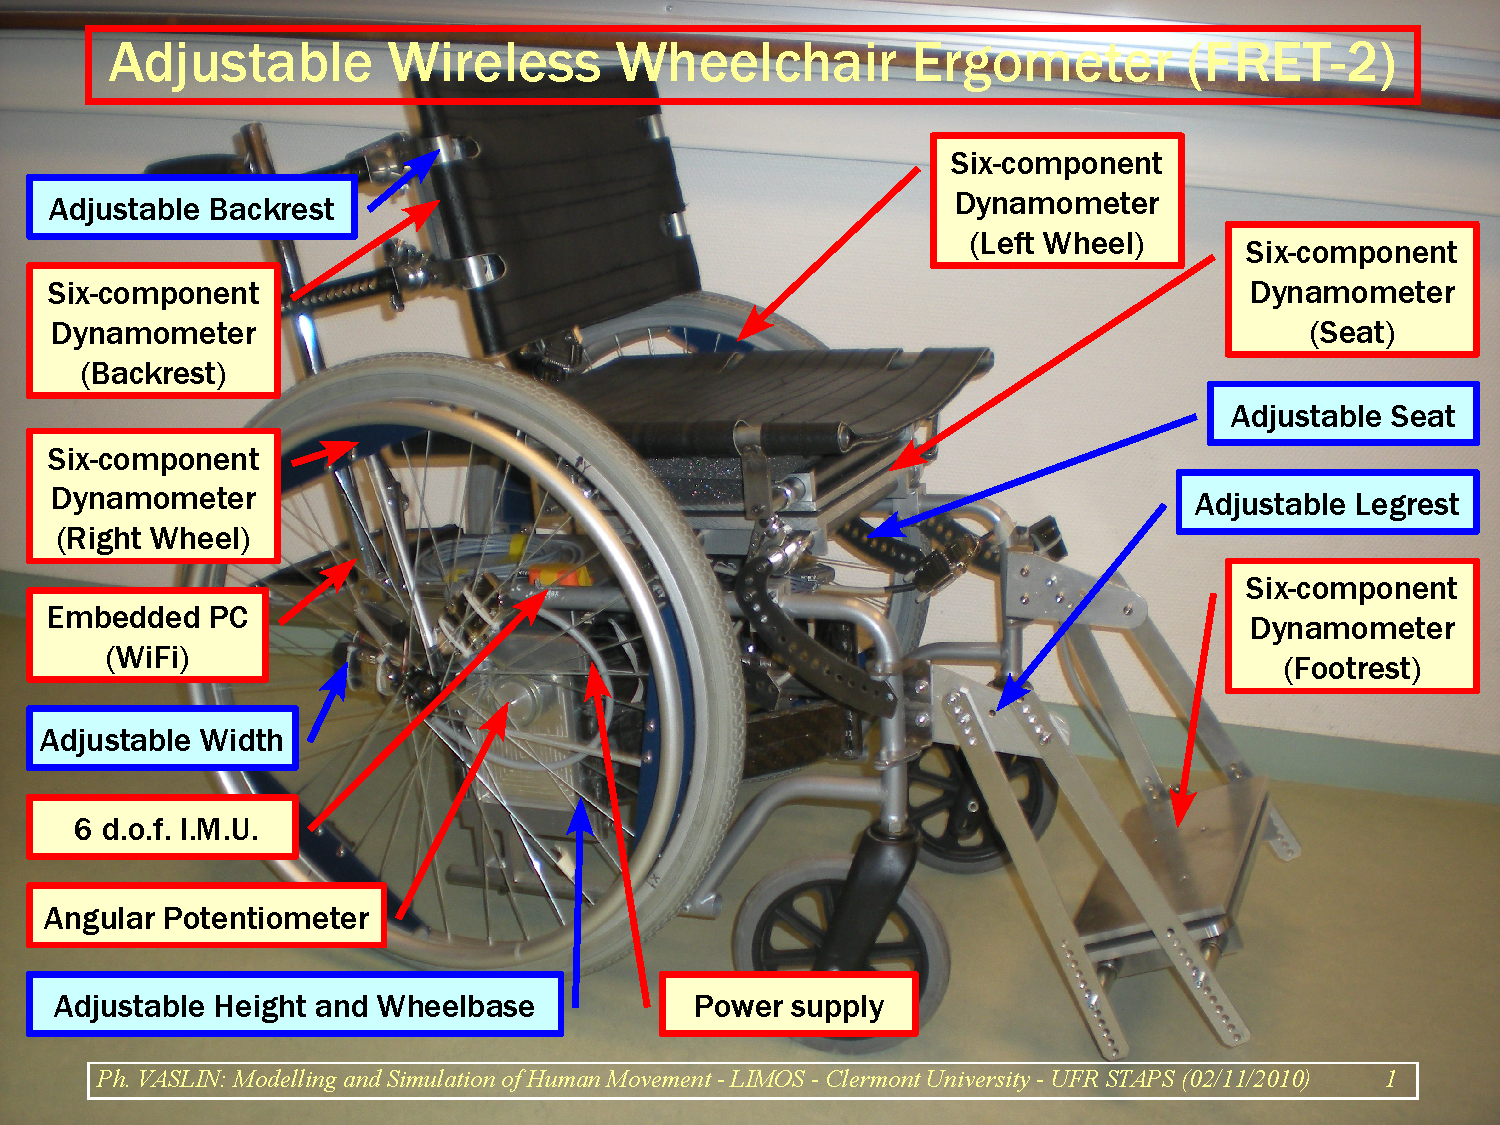
\includegraphics[scale = 0.4]{images/FRET-2_Legend_GB}
\caption{Captioned picture of the adjustable wireless wheelchair ergometer (FRET-2).}
\label{fret_legend}
\end{figure}


The measurements recorded by the sensors, which are the prupose of our analysis, consist of 41 attributes; of which 30 represent the dynamic parameters (Fx, Fy, Fz, Mx, My, Mz = 6 components x 5 dynamometers). The 11 other attributes represent the kinematic parameters of the MWC and its position relative to the Earth's magnetic North.

\subsubsection{The force and torque dynamometer}

A "torsor" is a mathematical object that characterizes the efforts applied on – or by – a solid. It is composed of two vectors, which have three components each: the three components (Fx, Fy, Fz) of the resulting force (F) and the three components (Mx, My, Mz) of the resulting moment (M) that are applied to this solid along three orthogonal axes (x, y, z). To measure the six components of the "torsor" applied by wheelchair users on both handrims during their actual displacements on the ground, an original force and torque dynamometer has been designed, built and installed on both rear wheels of the FRET-1 and then the FRET-2 (Fig. \ref{capteur_tri_axe}). This dynamometer is composed of three bidirectional force sensors that measure all the forces applied to the handrim which are then used to compute the three components of the resulting force and the three components of the resulting moment.

\begin{figure}[h]
\center
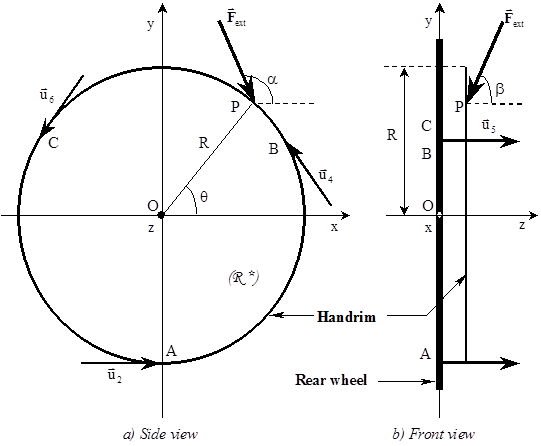
\includegraphics[scale = 0.35]{images/principle_six_component_sensor}
\caption{Schematic principle of the six-component force and torque sensor (patent WO 1995001556 A1) mounted of both rear wheels of the MWC field ergometer used in this study (FRET-2).
\\
\textbf{Legend}
\begin{itemize}
\item $R^{*} (O,\,x,\,y,\,z)$: moving reference frame linked to the wheel;
\item $O:$ centre of the wheelchair rear wheel;
\item $R:$ radius of the wheelchair rear wheel;
\item $A,\, B,\, C:$ locations of the three two-component force tranducers;
\item $u1,\, ... ,\, u6:$ unit vectors of the six force transducers;
\item $F_{ext}$: external force applied by the user on the handrim;
\item $P:$ point of application of Fext on the handrim;
\item Angles: $a = (u_x, F_{ext}); b = (u_z, F_{ext}); q = (u_x, OP)$ 
\end{itemize}
}
\label{capteur_tri_axe}
\end{figure}



The wheel dynamometer used in that study is based on a mechanical principle already applied for the design of a six-component dynamometer used for the measurement of the forces and torques applied by the pole-and-vaulter system in the vaulting box during the pole vault.

According to that principle, the handrim is assumed to be rigid and firmly fixed on three two-component force transducers designed to measure the handrim displacement with respect to the wheel. In that approach, the handrim is considered as hanging on the wheel through the force transducers. Each transducer measures one component of the resulting propulsive force in the tangential direction of the wheel and one in the direction perpendicular to the plane of the wheel. The vectorial sum of all these components is equal to the resulting propulsive force in the moving reference frame $R^{*}$ linked to the wheel. This derives from the fact that the handrim is static in $R^{*}$ with respect to the wheel.


When an external force Fext is applied on the handrim, it is instantaneously transmitted to the six force transducers so that each of them simultaneously measures a local force $F_i$ $(i = 1 \, to \, 6)$. As the transducers behave as springs, which stiffness $k_i$ are determined through the calibration procedure, the measurement of the displacements $m_i$ by the strain gauges allows to compute the values of $F_i$ using Hooke's law (equation \ref{eq:hooke})

\begin{eqnarray}
F_i = k_i m_i.
\label{eq:hooke}
\end{eqnarray}



Finally, the force and torque components created by $F_{ext}$ are calculated by equation \ref{eq:torseur}

\begin{eqnarray}

\overrightarrow{F}_{ext}=
\stackrel[i=1]{6}{\sum}\vec{F}_{i}\iff\left[F_{ext}\right]=
\left[k_{i}\right]\left[m_{i}\right]\iff\left[F_{ext}\right]=\left[\begin{array}{c}
F_{x}\\
F_{y}\\
F_{z}\\
M_{x}\\
M_{y}\\
M_{z}
\end{array}\right]

\label{eq:torseur}

\end{eqnarray}

Where $\left[F_{ext}\right]$ is a column matrix containing the six components of the torsor applied on the dynamometer; $\left[k_{i}\right]$ is the sensitivity matrix of the dynamometer;  $\left[m_{i}\right]$ is the column matrix containing the signals measured by the six forces transducers of the dynamometer.
Several mechanical and kinetic parameters can be computed from the forces and torques measured by the six-component dynamometers mounted on the MWC field ergometer \cite{Sauret2010}. All of them have a specific and useful meaning as their relationships are defined by a complete mechanical (i.e. dynamic and kinematic) model of wheelchair propulsion. However, because of their number and their complexity, these parameters can only be analysed and interpreted by specialists in biomechanics. To overcome this drawback, in the present study, relevant mechanical information has been extracted from only some dynamic data (z-moments $M_z$) recorded by both rear wheel dynamometers of the instrumented MWC (FRET-2) [This information have then been used to group subjects in homogeneous clusters, which have been compared to clinical injury levels.

\section[Wheelchair time series]{Knowledge discovery on wheelchair time series}
\label{mechanical_model}
After the construction of these measuring instruments (FRET-1 and FRET-2), they have been used to measure the efforts made by MWC uses in actual conditions of wheelchair locomotion. Thus, several experiments have been conducted with several subjects,  where the efforts produced during actual wheelchair locomotion were measured with the FRET-2. The abundance of the recorded measurements highlighted the problem of the exploitation of these measures for knowledge extraction. Two main and complementary approaches can be used to analyze measurements from MWC locomotion. The first is to use mechanical models to calculate the physical parameters of motion and the second is to use data mining models to exploit measurements.  In this section, we present the contributions of these two approaches, which will allow us to position our work.



\paragraph{}Manual wheelchair locomotion causes significant mechanical stresses in the upper limbs \cite{desroches2010expression}. To remedy this problem, biomechanical studies have been conducted to identify and quantify traumatic factors such as:
\begin{itemize}
\item The doctoral thesis of Nicolas DE SAINT REMY (2005) \cite{Remy2005} who proposed a
mechanical model relating the forces applied to a MWC and its displacement ( Figure \ref{Wheelchair_model} ). This work particularly highlighted the fact that wheelchair acceleration is a function of subject's movements.

\begin{figure}[h]
\center
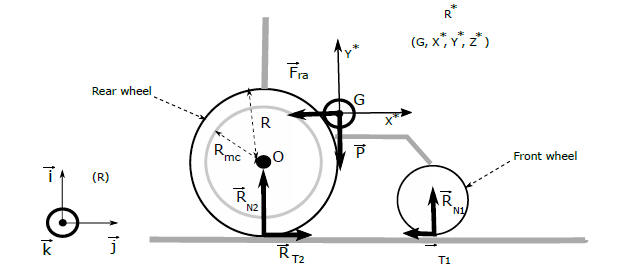
\includegraphics[scale = 0.65]{images/wheelchair_model2}
\caption{Balance of forces applied to a manual wheelchair during propulsion. For the clarity of the figure, the analysis of the movement of the \{subject + MWC\} system is reduced to that of the system's centre of gravity, G \cite{Remy2005}}
\label{Wheelchair_model}
\end{figure}

\item The doctoral thesis of Christophe SAURET (2010) \cite{Sauret2010} who proposed a method of calculating the mechanical power developed by manual wheelchair users to move. This model analyzes the kinetics of the \{subject + MWC\} system. For that purpose, the author developped a detailed kinematic model of the \{subject + MWC\} system (Figure \ref{Wheelchair_model2}) allowing to record their movements with a 3D motion analysis system during actual locomotion on the ground. 


\begin{figure}[h]
\center
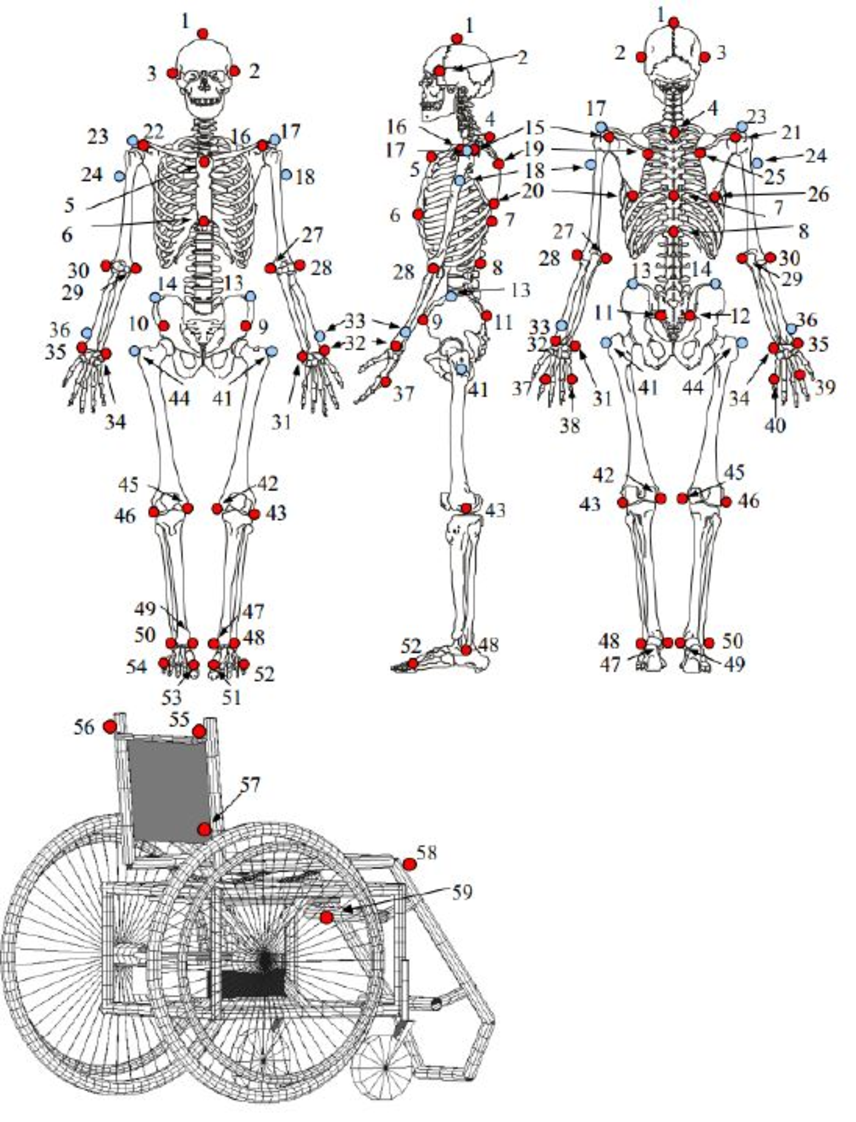
\includegraphics[scale = 0.5]{images/squelette}
\caption{Locations of passive markers for the kinematic analysis of manual wheelchair locomotion \cite{Sauret2010}}
\label{Wheelchair_model2}
\end{figure}

\end{itemize}


\paragraph{} More and more works in the literature suggest using the tools developed in data mining for a better understanding of human locomotion. For example, in \cite{van2017future}, the authors ask whether advances in data science and technology could provide a different and perhaps more objective view of the analysis of wheelchair users' motor abilities. On one hand, technical advances have made it possible to measure the efforts made by wheelchair users during their movement using sensors. On the other hand, datamining models have been proposed and allow to perform several task on the data (clustering, classification, …). 

In \cite{faria2012patient} the authors explained how they used robotics and data mining knowledge to build an Intelligent Manual Wheelchair, which can be controlled from multiple interfaces: joysticks, facial expressions, voice commands, head movements.  Since Intelligent Wheelchair users have various characteristics, a series of tests have been carried out to classify them and to define profiles that allow the MWC to be appropriately adjusted  for each user.

In \cite{athanasiou2009bayesian} the authors presented a model based on Bayesian networks to improve the medical treatment of patients in wheelchairs with a spinal cord injury. Indeed, the treatment of these patients  is based on the level of spinal cord injury and symptoms. A lesion in the spine has three consequences: an inconsistency of the bowel, an inconsistency of the bladder, a loss of the skin sensitivity. The higher the lesion, the more widespread its effects on patients are. Thus a patient with a low lesion will affect the patient's legs  and a patient with a high lesion will see his four limbs affected. Because of this loss of sensitivity, symptoms observed in the patient are often incomplete, which introduces uncertainty into the diagnosis that is captured by Bayesian networks and conditional probabilities.





\section{Conclusion}



Throughout this chapter, we showed that there is a large number of MWC users in the world and that it is crucial to analyze this particular means of locomotion to improve the living conditions of people moving in a MWC. We have presented the main tools designed and manufactured for wheelchair locomotion analysis and some previous works that used data mining mechanics models to improve the study of wheelchair locomotion or  to  help physicians to diagnose its the adverse effects. 


In the scientific literature,  mechanical or data mining models are used for manual wheelchair locomotion analysis.  In this thesis, however, we want to \textbf{design} data mining models that are able to take into account both the specificities of MWC locomotion data and their use to analyze wheelchair locomotion from a new point of view. 


%\chapter{Hellinger Based Distance for Uncertain time series}
%\label{helinger}
%Deterministic Measures like traditional similarity measures, return a real number as
%the distance between two uncertain time series. 






































